\chapter{Introduction}

\section{Overview}
\label{Intro: Overiew}

In recent years, Human-Computer Interaction (HCI) projects in sensitive contexts have considered how to best conduct and design research with people who might be regarded as vulnerable or positioned as part of marginalised communities \citep{waycott_challenge_2015}. One of these populations frequently designed \textit{for and with} are people with dementia \citep{suijkerbuijk_active_2019}. Dementia is a neurodegenerative condition that produces varying cognitive changes. Given that people may experience changes to their cognitive abilities, increasing need for care, and making judgements, many of the social and cognitive consequences of dementia can be framed as ethical concerns, making it a challenging space for both research and care practices \citep{herrmann_systematic_2018}.

Moving from an early, medicalised understanding of dementia as a process of decline and memory loss, recent social justice and rights-based responses to the experience of dementia have resulted in a more holistic understanding of the condition \citep{shakespeare_rights_2019}. This evolving understanding of dementia is mirrored in social and technological responses in research, which moved from early assistive technologies focusing on bridging a ‘cognitive gap’ \citep{mulvenna_supporting_2010}, to experience-centred design that fosters creative expressions of personhood \citep{morrissey_value_2017}, to more recent work on supporting wider social engagement with people with dementia \citep{foley_care_2019, lazar_safe_2019, welsh_ticket_2018}. Through understanding best practices for designing with and for people with dementia, HCI researchers have developed a range of approaches which centre on relational interactions, as opposed to engaging this population solely at the end of the design process, e.g., by inviting participants for ‘user testing’ or ‘user evaluations’ \citep{brankaert_intersections_2019,schorch_designing_2016, vines_designing_2013}. However, by providing a more relational approach in such work, researchers and participants face different challenges. For instance, \cite{hendriks_challenges_2014} describe the need for longer-term commitment to projects to support trustworthy relationships between the researcher and participants. Furthermore, the authors draw attention to the implicit decision-making designers and researchers may make because they have specific skillsets or expertise.

With the increase in multidisciplinary teams (e.g., encompassing designers, developers, and researchers), researchers have designed multiple approaches and design thinking activities to ensure designers and developers  \textit{``understand the design situation and the problem at hand and to explore and experiment with potential solutions.''} \citep[pg. 21]{dalsgaard2017instruments}. In the context of dementia and HCI, this has led to inviting students to collaborate in co-design methods with care home residents by developing life story work \citep{foley_student_2020} and storytelling projects \citep{hannan_zeitgeist_2019}. \cite{hendriks_valuing_2018} further support the importance of designers and students building a relationship with the people we are designing for and within the context of dementia. The authors argue design decisions \textit{``emerge from the relationships designers build''} \citep[pg. 3]{hendriks_valuing_2018}. However, while opportunities to work in more non-traditional settings such as care homes may be possible through university classes, these are often limited to a small, selected group of students or courses focusing on healthcare and psychology \citep{kinnunen_understanding_2018}, meaning those who are taught technical or design disciplines through university miss out on opportunities to gain experience with the vulnerable populations that they may end up building for.

This thesis explores \textit{``How might participation be configured for people with dementia to shape the design process of technology?''} Previous HCI research working closely with people with dementia stresses the need for method adaptability to ensure inclusive and meaningful engagement. In turn, this raises the question of what approaches should be considered for designers and developers that allow them to design with people with dementia collaboratively.This thesis describes four studies involving diverse stakeholders' perspectives who are commonly part of the design process when designing for and with people with dementia. Each study iteratively explores the competing interests and expectations of involving a diverse group of stakeholders to collaborate in the design process. These studies' findings and discussion sections contribute new knowledge concerning how participation is adapted and shaped to develop inclusive design spaces that support mutuality in creating new technologies and systems.

\section{Research context}
\label{Intro: ResearchContext}
To provide an understanding of technology design in the context of dementia, the research context is split into the following: 
\begin{itemize}
\item \textbf{Continuing to experience the world with dementia:} Moving from an early, medicalised understanding of dementia as a process of decline and memory loss, dementia research and care practices have resulted in approaches to ensure the person with dementia is respected and engaged.

\item \textbf{Technology and dementia:} This evolving understanding of dementia is mirrored in technological responses, which moved from early assistive technologies, to designs that foster creative expressions of personhood, to more recent work on supporting broader social engagement with people with dementia.


\item \textbf{Learning about dementia through design:} To help foster empathy with, and understanding of, a person with dementia's experience, HCI work have developed novel approaches to upskill design team's processes.

\end{itemize}


\subsection{Continuing to experience the world with Dementia}
\label{Context:Dementia}
Historically, dementia has often emphasised its biomedical origins \citep{lyman_bringing_1989}. As dementia progresses, it often adds conflict between the person and their surroundings as they can become unfamiliar, and this can also cause difficulties with coexisting with others; this can happen in what was previously a familiar space such as a family home, a local community, or work place \citep{langdon_making_2007}. People with dementia can find themselves feeling stigmatised within new roles or of `patient', `demented', and `in need of care' \citep{cohen-mansfield_utilization_2006}. This can create social exclusion by depriving the person with dementia of their personhood and changing their quality of life \citep{lawrence_improving_2012}. The progression of dementia means that the individual's role within the family structure can change, as they become the care-receiver, and therefore, the impact of dementia can be troubling for both parties \citep{dupuis_moving_2012}. In particular, social activity can decrease, which entails several `knock-on' effects, such as a decline in emotional well-being, and increased social isolation and depression \citep{bartlett_citizenship_2014}. 

In response to the medicalisation of the experience of dementia, person-centered approaches have highlighted the need for socially-oriented care, in which the individual is positioned central to the advancement of their care \citep{bond_medicalization_1992,manthorpe_person-centered_2016}. In the 90's \cite{kitwood_towards_1992} promoted the concept personhood in care that proposes a series of person-centred approaches to acknowledge the entire individual to ensure they are heard, included and understood. Since then, many researchers have built upon and used person-centred approaches to dementia care and have called attention to how we communicate with people with dementia \citep{oyebode_mental_2005}, debated the need for ongoing consent processes \citep{dewing_participatory_2007}, and promoted the need to attune to embodied, non-verbal communication \citep{group_patron_2019, twigg_dress_2013} as key considerations in ensuring the person with dementia is respected and engaged within their own care. These practices, largely initiated within nursing and social care, have implications for research and design that seeks to work with and for people living with dementia, and to avoid practices that devalue or disregard the experience of the person living with dementia. \cite{john_killick_claire_craig_creativity_2012} highlight the use of arts and creativity to provide alternatives to verbal communication that demonstrate unique ways for people with dementia to share their experiences. Through humour, dancing, acting, music, movement, and fashion, people with dementia can communicate and share experiences that move beyond verbal communication.

While recognising the person with dementia's individuality has raised awareness in respecting the needs, wants and desires of the person with dementia, \cite{bartlett_personhood_2007} suggest embedding person-centred values within a citizenship lens that integrates a more socio-political and critical understanding of dementia. In particular, the lens recognises the challenges of stigma, relationship dynamics, and unique nature of the individual are all connections we must consider when reflecting on the dementia context. Moving towards a citizenship model has empowered and promoted people with dementia to share their experiences to make themselves more visible to impact policymaking, practice, and research \citep{weetch_involvement_2020}. For instance, \cite{bryden_challenging_2020}, a pioneering dementia advocate, has written many blog posts, presentations, and personal books advocating for changes in media and public portrayals of dementia in an attempt to change dominant misconceptions about, and stereotypes of, the condition. The sharing of experiences has an impact in two ways. First, advocating and sharing experiences fosters purpose and impact in understanding dementia on a more inclusive level; and two, the stories promote awareness and improve public perception \citep{reynolds2017stigma}.

To an extent, improving public perception and citizenship approach resonates with policy and practice. In 2020, the UK set out the Prime Minister’s challenge to make England the best place to live with dementia, and be the leading place in the world for dementia research \citep{budgett2021designing}. This challenge set out to tackle: dementia-friendly health and care settings; educating people earlier about the risks of developing dementia; and  providing more opportunities for people with dementia to partake in research and present talks about their experiences. \cite{keady2017social} argues that these aims by the UK present dementia as \textit{``everyone’s business and responsibility, from architects to town planners, public transport providers to shop owners, next-door neighbours on the street where the person with dementia lives - the list is seemingly endless''}. As such, given that dementia is part of a complex ecology of care, which considers the person with dementia, friends, family, healthcare systems, researchers, designers, and everyday interactions, it is particularly timely to unpack what it means to design methodologies that consider the multivariate stakeholders and infrastructures that surround and often hold up our work. 

\subsection{Technology and dementia}
\label{Context:Design}
Similarly, technology design and dementia solutions initially focused on cognitive decline, monitoring and management. This focus resonates with the biomedical approach to care, which assumes the experience of dementia is only concerned about the neuro-cognitive condition and decline in abilities \citep{o2022conceptualizing}. This early work in technology design considers using sensors, surveillance technology, and devices to compensate for the physical and cognitive deficits of people with dementia. While these technologies might provide people with dementia with freedom of movement and improve quality of life, \cite{bharucha2009intelligent} reports that these early studies would be often guided by family and professional care staff instead of people with dementia. In turn, this has knock-on effects where the technology used by people with dementia does not consider their needs. For instance, \cite{astell2006technology} reports on how tracking technology may devalue the person with dementia's agency by care partners or staff being able to track and follow where the individual is going. This particularly becomes challenging where monitoring technology may reduce human contact between the person with dementia and the care partner. In this way, \cite{astell2006technology} argues that these ethical issues in early work in the area of HCI and dementia largely stem from the lack of involvement of people with dementia in the design process to understand their needs and interest in technology.

The lack of involving people with dementia in the design processes comes from the challenges of verbal communication \citep{majlesi2017video}, potential stress research may cause, and researchers being unaware of such biases, which may assume people with dementia lack the capability to contribute to the design processes \citep{manthorpe_person-centered_2016}. As HCI began to extend person-centred approaches to dementia, studies such as CIRCA \citep{astell_stimulating_2010} and KITE \citep{robinson2009keeping} challenged the role that people with dementia play in the design process of technology. Through these initial studies, researchers adapted their methodologies to centre the voices of people with dementia, supporting tailoring the user's assistive needs. 

From here, HCI research in dementia is a growing body of work that relies on relational processes as the basis of design. This has resulted in the introduction of technologies that evoke emotion \citep{wallace_enabling_2012-1,houben_foregrounding_2019,dixon_approach_2020} , engage in creativity \citep{lindsay_empathy_2012,morrissey_im_2016} and support inclusion \citep{welsh_ticket_2018,foley_printer_2019,treadaway_sensor_2016}. For instance, \cite{wallace_design-led_2013} use a tailored approach that centred the importance of personhood by paying attention to a person’s individual and unique experiences of dementia to design bespoke digital artifacts for the participants. Similarly, \cite{lindsay_empathy_2012} describes the need for more interpretative data approaches for those at later stages of dementia, which in turn, may require longer-term projects and relationships to form throughout a study. This early work stresses the required need to adapt co-design and participatory approaches to accommodate the differing communication needs of people with dementia, ensuring they are respected rather than infantilised \citep{brankaert_intersections_2019}. 

More recent work has seen a critical turn to understanding personhood even in the presence of later stages of dementia, where non-verbal and ambiguous interactions may be more present \citep{lazar_critical_2017}. \cite{treadaway_sensor_2016} emphasise that recognition and appreciation are crucial even when leaning on tacit, creative activities to support non-verbal interactions. This critical turn is further supported in work by \cite{morrissey_value_2017}, taking an experience-centred approach that shifts the way we see people with dementia-related cognitive deficits as contributing to design choices. While prior work may focus on alleviating a person's cognitive deficit, the critical perspective widens our approach to inclusivity, by celebrating what a person has to offer through more creative and engaging approaches, where those living with a broad spectrum of dementia-related changes can also participate \citep{foley_printer_2019}.

\subsection{Learning about dementia through design}
\label{Dementia-Design}
Given the growth in multidisciplinary teams to develop and design technology, researchers have considered novel approaches to undergraduate education to provide budding designers and developers with the skillset and ethics to make more sensitive design choices. In the context of dementia and HCI, this has led to inviting students to collaborate in co-design methods with care home residents by developing life story work \citep{mckeown2015you} and storytelling projects \citep{hannan_zeitgeist_2019}. 

%% Needs rewriting
\cite{hendriks_valuing_2018} further supports the importance of designers and students building a relationship with the people we are designing for and with in the context of dementia. The authors argue design decisions \textit{``emerge from the relationships designers build''} \citep[pg.3]{hendriks_valuing_2018}. However, while opportunities to work in more non-traditional settings such as care homes may be possible through university classes, these are often limited to a small, selected group of students or courses focusing on healthcare and psychology \citep{kinnunen_understanding_2018}, meaning those who are taught technical or design disciplines through university miss out on opportunities to gain experience with the vulnerable populations that they may end up building for. Finally, developing these types of understandings through intergenerational interactions has often relied on organisations or care homes to provide a community of older adults or people with dementia, both increasing the workload of already pressured social care organisations, and limiting the potential of involving communities or individuals who are not part of those selected organisations. 

Alternatively, researchers have often developed toolkits and other creativity support mechanisms to support empathy-based skill development for individuals implicated in the design process. For instance, \cite{chen2020interaction} introduce a toolkit for turning conference papers into actionable guidelines and design tips through the curation activity of undergraduate researchers, who review papers and summarise the key findings down into a series of guidelines. However, the use of design toolkits can face challenges where other cultural contexts and settings interact \citep{peters2020toolkits}, such as when values, goals and technologies displayed on cards may have little to no meaning within the setting. While one approach is to make toolkits more abstract and open to be applicable for different settings, \cite{peters2020toolkits} suggest tools be more \textit{``consciously culturally-tailored''}.  

It is clear that creating specialised toolkits for use in particular settings or contexts requires specialist input to ensure the content is appropriate \citep{alshehri2020scenario,meissner2018schnittmuster}. For example, \cite{craig2021development} developed an ethical roadmap for designing at the end-of-life; this roadmap comprised components such as value cards, ‘informedness’ of consent questions, provocations, and value cards to support developers and designers to reflect on and question their approaches to this very contested area of work. To curate the cards and content for the ethical roadmap, the authors worked with a diverse team of experts in end-of-life matters, digital media, and physical object design, as well as with participants whose experiences in bereavement spoke to the toolkit’s use. In a similar study, \cite{shinohara2020design} describe a series of design cycles requiring various stakeholders to develop a set of method cards for social accessibility. While \cite{shinohara2020design} emphasises the toolkit should not replace students directly speaking to users, they explain that the toolkit provides \textit{``information about how to interact with expert users''} and that this \textit{``helped students to know how to start conversations and guide them toward productive discussions'}'. In turn, this raises the question of what sorts of toolkit interactions we should provide to designers and developers that allow them to collaboratively design with people with dementia while at the same time, prioritising speaking and involving people with dementia.

\section{Thesis structure}
\label{Intro: Thesis structure}
To understand how this thesis tackles \textit{``how might participation be configured for people with dementia to shape the design process of technology''}, the following section describes the structure of the thesis. Following this section, I return to the research aim and describes how it is split into three questions to explore participatory design, ethical implications for participation, and competing interests and desires from diverse stakeholders. 


\subsection{Chapter two - Background Literature}
\label{Intro:ChapterTwo}
This chapter describes prior work on the representation and involvement of people with dementia in technology design and development. Initially, this chapter reviews the involvement of people with dementia in HCI work that draws attention to building relationships between researchers and participants and iterative design processes to demonstrate that participants are being listened to and influencing the design. Following the review of HCI work in the context of dementia, I highlight three knowledge gaps. The first is that HCI work has primarily focused on mild to moderate stages of dementia for participation, resulting in an unrepresentative perspective of involving people with dementia and stakeholders in technology design. Second, while researchers have raised several ethical complexities in this domain, the dementia context in HCI is still somewhat new and could benefit from reviewing non-HCI dementia work to understand their everyday ethics for working with people with dementia. Third, given the relatively recent work in dementia and HCI on tackling dementia public awareness \citep{lazar_safe_2019,talbot_how_2020}, there is an opportunity to understand how we might support the teaching and dialogue on dementia awareness for technologists who are ultimately the ones making design decisions on behalf of people with dementia.  

To extend my understanding of these missing gaps, I draw from outside the HCI literature to examine the type of ethical dilemmas; public perception of dementia and involving later stages of dementia in the co-creation process. Finally, to conclude this chapter, I describe four areas of interest to this thesis that shape the thesis. The four areas are the following: 
\begin{itemize}
    \item Attending mutual collaborative relationships
    \item Representation of technology and dementia from a designer/developer perspective
    \item Ethical practice in dementia-HCI
    \item Promoting learning around dementia and technology
\end{itemize}

\subsection{Chapter three - Methodology}
\label{Intro:ChapterThree}
In the methodology chapter, I explain and justify the research approach taken in the thesis that shapes the data chapters. First, I introduce the epistemological approach, which from my understanding, is a social constructionist approach in which the creation of knowledge is a collaborative process. Following, I unpack participatory methods in dementia and HCI that emphasise the need to adopt approaches to fit the needs of people with dementia. I then describe how I adapt co-design and participatory design to fit the needs of people with dementia. The chapter presents discussions regarding the ethical challenges of the thesis; ways I captured data; recruitment and location details; and the qualitative data analysis method, thematic analysis. To conclude the methodology chapter, I describe the process of reflexivity, validity, and reliability to support the data analysis process. 

\subsection{Chapter four - Sharing a Virtual World with People with Dementia: A Reflective Account}
\label{Intro:ChapterFour}
The chapter is a reflective account of two studies working with a dementia café to design VR and media experiences with and for families with dementia. I worked closely with a dementia café in Newcastle called Silverline Memories, which provides activities and organises celebrations for members’ birthdays and other special occasions. By working closely with families with dementia, the account examines how I adapted participatory approaches to involve people with dementia in more sensitive and meaningful ways. For instance, given that some members of the families were rarely verbal, I used walking interviews as an opportunity to observe their interactions and listen to their stories if they chose to share. 

Further, by working with family members as well as the person with dementia, I recognise that many of the challenges in designing technology with people with dementia should consider the needs and interests of the ecology of care. In that respect, this chapter takes a reflective approach to provide a clear account of my background, history, my perspective on dementia, and design approaches that ultimately impact the participants, the setting, and the overarching work. As such, this chapter provides insights into designing VR environments for families with dementia within a personal narrative that recognises the concerns, dilemmas, and the impact of working within sensitive research spaces. In response to the lessons learned, the following two chapters examine: a) designers'/developers' shifting sensitivities about dementia in a hackathon aimed to provide a space for upskilling attendees on HCI and dementia, and b) the types of ethical concerns HCI researchers face in the dementia context. 

\subsection{Chapter five - DemVR: Exploring Shifting Sensitivities in a Hackathon for Dementia}
\label{Intro:ChapterFive}
Following chapter four, which focused on the inclusive design of virtual reality experiences for families living with dementia, at the time, local authorities were interested in extending this work to larger groups of people through public-facing events - such as a hackathon. At the same time, this interest prompted me to explore how inclusive design might function within the context of larger-scale community events, which was in stark contrast to my prior work that required working closely with participants.

The event consists of two stages: a six-week engagement phase to support participants in proposing and refining initial ideas online; and a two-day hackathon inviting designers and domain experts to develop their ideas further. While the event gained reasonable interest from designers, developers, and students throughout both phases, the representation of people with dementia and their care partners was limited. The chapter examines the structure of the event and the role this played in the struggle to involve people with dementia and their care partners. The data analysis presents insights into participants’ motivations, design approaches to accommodate the absent user, and the design ideas that the teams developed to address the social context of the user. Against a background of the extant literature on reification in design, collaborative design events, and dementia, the discussion provides a series of commitments for HCI and dementia research. The commitments offer insights into how we might mitigate stereotypes in constructing the end-user; ways to improve recruitment for involving marginalised populations in events; and steps to promote more inclusive, community-driven events. 

\subsection{Chapter six - Learning from Ethics in Dementia Research}
\label{Intro:ChapterSix}
In chapters four and five, I describe engaging in participatory research in HCI raises numerous ethical challenges such as research relationships, participant recognition, recruitment and consent. Doing HCI work in sensitive settings amplifies these issues, and researchers in this area are modelling approaches to ensure participants are meaningfully engaged and represented in their work. In response to this need, HCI researchers are reflecting on the ethical challenges they face throughout their research process \citep{vines_designing_2013}, with conversations largely occurring in venues such as Town Halls \citep{munteanu_sigchi_2019,bruckman_cscw_2017} and conference workshops at ACM venues \citep{davis_ethical_2015,waycott_challenge_2015}.

In this chapter, I take design ethics in dementia and HCI research to elucidate broader concerns about ethics and HCI when doing design research with people with dementia and their care partners. I interviewed 22 researchers from diverse countries, institutions, and work in dementia design research. The analysis examines the potential challenges researchers face with Ethical Review Boards (ERB), who, while prioritising the protection of human subjects, can inadvertently bar the full inclusion of people living with dementia in socially-oriented research. Researchers also shared insights from their own cultivated practices from establishing clear expectations for participants, knowing when and how to involve participants in the research, and appropriately acknowledging the contribution that participants make to our work. I proceed from the findings to emphasise a set of directions for researchers and ethical review boards to improve their practices by moving towards more participant-led research, re-framing impact and aiming for research clarity.

\subsection{Chapter seven - Co-creating a Digital Toolkit to Support Design for Dementia}
\label{Intro:ChapterSeven}
From the previous two chapters, it was apparent that: 
\begin{itemize}
\item Representing people with dementia can be difficult in public events and causes multiple knock-on effects on design outputs.
\item Future research work in dementia should aim to be participant-led and shift towards creating tools or processes to promote conversations between people with dementia and stakeholders commonly implicated in design processes.
\end{itemize}

The two chapters question how can we support collaboration and engagement between those who are being designed for, and those who are doing the designing. To explore the needs and desires of the diverse set of stakeholders, this chapter presents the design of the Dialogical Dementia Design (D3) toolkit, a set of resources to support co-designing with people with dementia. I invited 11 developers, designers and five people with dementia for a series of interactive workshops and interviews that explored resources needed by developers and designers to design with people with dementia and investigate how people with dementia envision their potential participation with toolkits. The analysis raises questions about the challenges of co-creation through safety and privacy, the sharing of the ‘designer’ role between the different stakeholders, and finally, the type of incentives required for participation and engagement in curating a toolkit. Finally, this chapter concludes with insights into highlighting how we might balance participants' privacy, safety, and due recognition; priorities in growing a community-owned toolkit; and the accountability and responsibility designers and developers carry in adapting their working practices for designing within sensitive areas.

\subsection{Chapter eight - Discussion and Future Work}
\label{Intro:ChapterEight}
In the closing chapter, I synthesise the findings from the data chapters and revisit the research questions I set out at the start of this thesis. The discussion aims to answer how researchers adapt participation approaches to provide more engaging experiences for people with dementia; how, as researchers, can we mitigate some of the ethical implications for when people with dementia participate in HCI research; and how can we balance and design for the competing interests and expectations of diverse stakeholders to ensure the support of meaningful dialogue between people with dementia, designers, and developers. 

The chapter concludes with a future work design approach consisting of three core components that reimagine the role of participation between people with dementia and stakeholders. These three components consider a) an inquiry panel of expert stakeholders to guide and shape research agendas and provide support through the running of a study; b) three critical areas of impact that researchers must consider when starting a project; and c) a set of three considerations to articulate stakeholder interests and priorities through the research process. By considering the three components, the approach aims to move towards more inclusive design spaces that support mutuality in the co-creation of new technologies and systems.

\section{Research aim and questions}
\label{Intro:RQ}
The research described in this thesis explores the following research aim:
\begin{quote}
    \textit{``How might participation be configured for people with dementia to shape the design process of technology?''}
\end{quote}
This research aim is split into three research questions, to provide insights into the experiences and perspectives of stakeholders commonly implicated in design processes in designing with and for people with dementia, intending to broaden the conversation surrounding technology design with and for people with dementia. The following section introduces each research question followed by a description.

\subsection{Research question one}
\label{RQ1}
\begin{quote}
\textit{``How can we use participatory design approaches to provide meaningful and engaging experiences for people with dementia?''}
\end{quote}
In exploring this question, the methodologies used in this thesis explore the ways to move toward more inclusive design approaches that require flexible configuration to support the unique needs of participants. Chapter four presents novel ways such as walking interviews that support people with dementia to talk about what is important to them, not only their personal history. Further in chapter five, the analysis of the hackathon demonstrates the challenges in using participatory design with people with dementia. The discussion raises essential insights into ways to improve recruitment for involving people with dementia and steps to promote more inclusive, community-driven events. Finally, chapter seven explores resources developers and designers need to design with people with dementia and investigates how people with dementia envision their potential participation with toolkits. Through this chapter, the analysis and discussion provide an understanding of how people with dementia want to share the 'designer' role and that incentives are necessary for participation and engagement. This exploration draws attention to how we talk about dementia, to what extent people with dementia want to contribute to technology design, and ways to ensure the person with dementia is respected and engaged in research.

\subsection{Research question two}
\label{RQ2}
\begin{quote}
\textit{``What are the ethical implications for people with dementia to participate in HCI research?''}
\end{quote}
Given that people with dementia may experience changes to their ability to problem solve, increasing need for care, and make judgements, many of the social and cognitive consequences of living with dementia can be seen as ethical challenges, making it a complex space for research. In chapters four and five, I reflect on the ethical challenges of establishing clear expectations for participants, knowing when and how to involve participants in the research, and appropriately acknowledging participants' contribution to the work. From these rich findings, chapter six closely examines ethical practices used in dementia and HCI research to present insights into the careful ethical considerations required when working with people with dementia and their families.

\subsection{Research question three}
\label{RQ3}
\begin{quote}
\textit{``What are the competing interests and expectations to support meaningful dialogue in dementia design research when involving multiple stakeholders - such as people with dementia, developers, designers and researchers?''}
\end{quote}
For the final research question, the thesis investigates the importance of designing for multiple interests and workflows to ensure that stakeholders who are part of the design process to support collaboration and engagement between the diverse stakeholders. Each chapter builds on answering this research question through exploring the interactions between people with dementia and the different stakeholders. For instance, these four chapters involve the following diverse set of stakeholders:
\begin{itemize}
\item Chapter four: people with dementia, care partners, family members, and friends
\item Chapter five: care partners, designers, developers, and undergraduate students
\item Chapter six: designers and researchers
\item Chapter seven: designers, developers, and people with dementia
\end{itemize}

By working with a diverse set of stakeholders, each chapter builds knowledge on how to balance and respect each stakeholder's different interests and expectations to move towards designing more inclusive and support spaces where people with dementia can contribute to co-creating new technologies and systems.

\newpage
\subsection{Thesis map}
For chapters four to seven, I present a map of which research question's each data chapter tackles (see figure \ref{fig:RQ_and_Chapters}).

\label{Intro:Thesis Map}
\begin{figure}[htp]
\centering
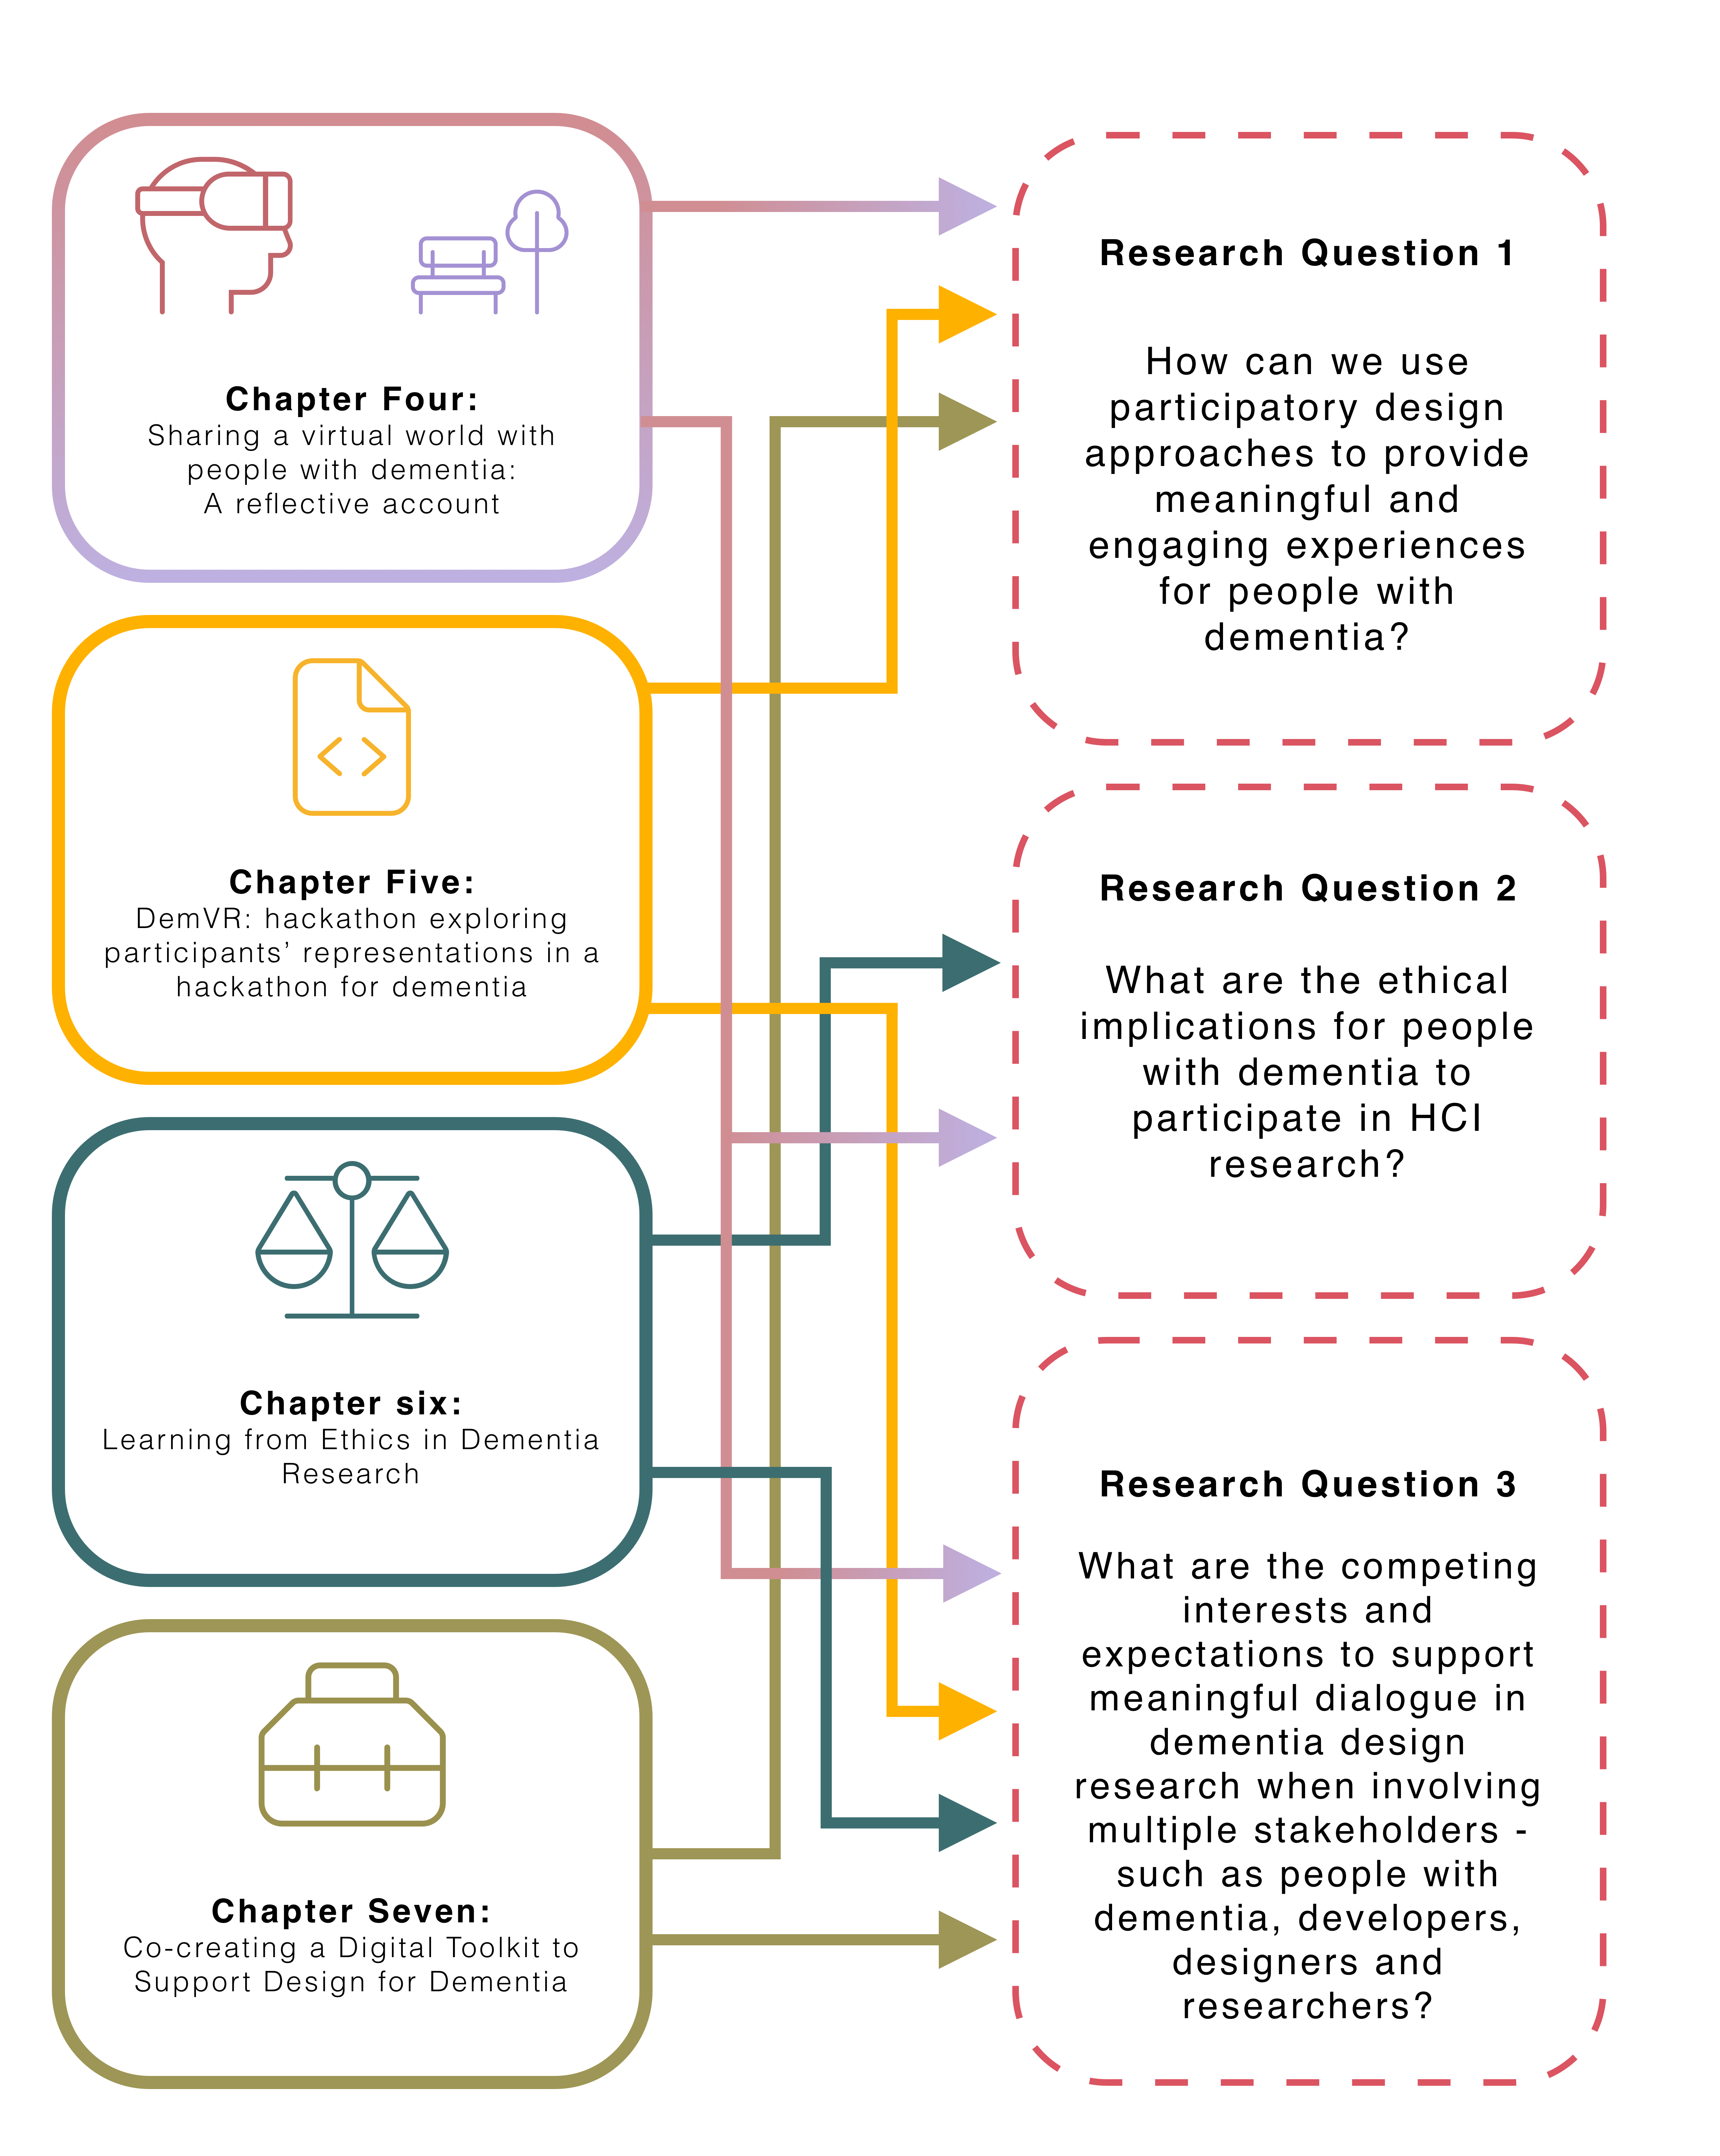
\includegraphics[width=.8\linewidth]{Images/Thesis_Narrative/RQ_and_Chapters.png}
\caption{Thesis Map showing the relationships between data chapters to research questions}
\label{fig:RQ_and_Chapters}
\end{figure}


\section{Contributions}
\label{Intro:Contribution}
In addition to the thesis resulting in a number of publications (see x), the thesis offers three contributions to knowledge in dementia and HCI:

\begin{itemize}
    \item \textbf{Empirical contribution}: This thesis uses data collected through walking interviews, workshops, a hackathon event, semi-structured interviews, and a three-stage iterative design process to provide qualitative insights into the experiences and perspectives of diverse stakeholders implicated in design processes in designing with and for people with dementia. Through characterising the distinct motivations and challenges faced by bridging communication between stakeholders, insights gained across the thesis reimagines the role of participation between people with dementia and stakeholders to promote conversation and inclusion of stakeholders in the technology design process. Each study offers practical examples of ways to create spaces to facilitate and support actively understanding and representing the contributions of people with dementia. 

    
    \item \textbf{Artefact contribution}: Within the thesis, two chapters present novel systems and prototypes to facilitate new insights and consider ways for people with dementia to engage with technology and contribute to the design process. In chapter four, I use the design of virtual reality environment prototypes to explore the ways people with dementia might use this novel technology. Through this work, the prototypes provide an understanding of the desire for shared experiences and how the sensitive capture and curation of digital media can help to keep the experience alive for people with dementia who might seek to experience such media `in the moment', in shared social contexts.
    
    In chapter seven, I collaborated with designers, developers, and people with dementia to develop a lo-fi prototype toolkit to support designers and developers in co-design with people with dementia. The main contribution of this is a series of directions for HCI and dementia research highlighting how we might balance participants’ privacy, safety, and recognition; ways for stakeholders to contribute to and grow a community-owned toolkit; and the accountability and responsibility that designers and developers carry when designing in sensitive and ever-changing situations.

    
    \item \textbf{Methodological contribution}:  The thesis contributes to a methodological understanding of how to support an equal relationship between those who are being designed for, and those who are doing the designing. In chapter four, by inviting families to a set of walking interviews (also known as days out), the families could communicate in ways beyond verbal interaction by taking the lead of the walk and using non-verbal expression to contribute to the research. For instance, I provide insights on the possibility of people with dementia self-regulating the flow of the day and expressing when they want to share their experiences and thoughts.

    Chapter five reports on the methodological challenges of recruiting people with dementia and care partners through online engagement platforms. The discussion emphasises an approach to meet participants where they are by considering the platforms they use, including the importance of offline engagement for those without technical abilities. As such, reflecting on how the approach led to a lack of involvement by people with dementia, this chapter provides ways to improve recruitment for involving marginalised populations in hackathons.
\end{itemize}
